% =============================================================================
%  Full Pipeline Walkthrough: process_after_rotation
%  Source → Transition System → Heap Model → Barrier → SMT → Bug Report
%  Bug class: DIV_ZERO (division by zero via floating-point norm collapse)
%
%  Every stage was executed by the A3 instrumentation script
%  (scripts/rotation_pipeline_instrument.py) and Z3 4.x.
% =============================================================================
\documentclass[aspectratio=169]{beamer}
\usetheme{metropolis}
\usepackage{appendixnumberbeamer}
\usepackage{amsmath,amssymb}
\usepackage{tikz}
\usetikzlibrary{arrows.meta,positioning,shapes.geometric,calc,
  decorations.pathmorphing,backgrounds,fit,automata}
\usepackage{listings}
\usepackage{booktabs}
\usepackage{xcolor}
\usepackage{fontawesome5}
\usepackage{mathtools}

% ── Color palette (matches barrier_transition_system_example.tex) ─────────
\definecolor{accent}{HTML}{2563EB}
\definecolor{accentdark}{HTML}{1E40AF}
\definecolor{safe}{HTML}{059669}
\definecolor{unsafe}{HTML}{DC2626}
\definecolor{warn}{HTML}{D97706}
\definecolor{bg}{HTML}{F8FAFC}
\definecolor{codebg}{HTML}{F1F5F9}
\definecolor{hilbert}{HTML}{7C3AED}
\definecolor{control}{HTML}{EC4899}
\definecolor{verify}{HTML}{0891B2}
\definecolor{taint}{HTML}{E11D48}
\definecolor{clean}{HTML}{059669}
\definecolor{fence}{HTML}{7C3AED}

\setbeamercolor{frametitle}{bg=accent,fg=white}
\setbeamercolor{progress bar}{fg=accent}
\setbeamercolor{alerted text}{fg=unsafe}

\lstset{
  basicstyle=\ttfamily\scriptsize,
  breaklines=true, frame=none,
  backgroundcolor=\color{codebg},
  keywordstyle=\color{accentdark}\bfseries,
  commentstyle=\color{safe!80!black},
  stringstyle=\color{unsafe!80!black},
  showstringspaces=false,
  numbers=left, numberstyle=\tiny\color{gray},
  escapeinside={(*@}{@*)},
}

\title{\textbf{From Rotation Loop to Safety Certificate}}
\subtitle{A complete barrier-theoretic walkthrough for \texttt{process\_after\_rotation}}
\author{A3 Python Analysis Engine}
\date{}
\setbeamertemplate{navigation symbols}{}

\begin{document}

% ═══════════════════════════════════════════════════════════════════════════
%  TITLE
% ═══════════════════════════════════════════════════════════════════════════

\begin{frame}[plain]
\titlepage
\end{frame}


% ═══════════════════════════════════════════════════════════════════════════
%  OVERVIEW
% ═══════════════════════════════════════════════════════════════════════════

\begin{frame}{Pipeline Overview}
\begin{center}
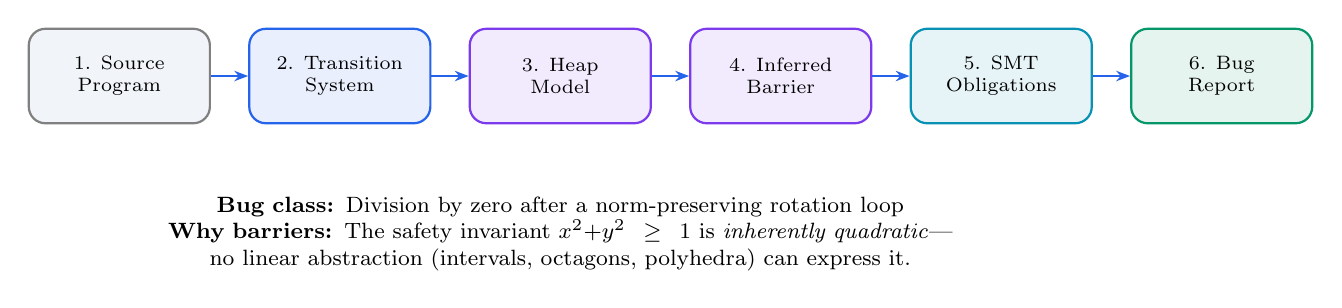
\begin{tikzpicture}[
  box/.style={draw, rounded corners=6pt, thick, minimum width=2.3cm,
              minimum height=1.2cm, align=center, font=\scriptsize},
  arr/.style={-{Stealth[length=5pt]}, thick, accent}
]
  \node[box, fill=codebg, draw=gray]   (src) at (0,0)    {1. Source\\Program};
  \node[box, fill=accent!10, draw=accent]   (ts)  at (2.8,0)  {2. Transition\\System};
  \node[box, fill=hilbert!10, draw=hilbert] (heap) at (5.6,0)  {3. Heap\\Model};
  \node[box, fill=fence!10, draw=fence]    (bar) at (8.4,0)  {4. Inferred\\Barrier};
  \node[box, fill=verify!10, draw=verify]  (smt) at (11.2,0) {5. SMT\\Obligations};
  \node[box, fill=safe!10, draw=safe]      (rpt) at (14,0)   {6. Bug\\Report};

  \draw[arr] (src)  -- (ts);
  \draw[arr] (ts)   -- (heap);
  \draw[arr] (heap) -- (bar);
  \draw[arr] (bar)  -- (smt);
  \draw[arr] (smt)  -- (rpt);

  \node[below=0.8cm of heap, font=\footnotesize, text width=12cm, align=center] {
    \textbf{Bug class:} Division by zero after a norm-preserving rotation loop\\
    \textbf{Why barriers:} The safety invariant $x^2{+}y^2 \ge 1$ is \emph{inherently
    quadratic}---no linear abstraction (intervals, octagons, polyhedra) can express it.
  };
\end{tikzpicture}
\end{center}
\end{frame}


% ═══════════════════════════════════════════════════════════════════════════
%  PART I — THE SOURCE PROGRAM
% ═══════════════════════════════════════════════════════════════════════════

\begin{frame}[fragile]{Stage 1: The Source Program}
\begin{columns}[T]
\begin{column}{0.55\textwidth}
\begin{lstlisting}[language=Python, title={\texttt{rotation\_target.py}}]
def process_after_rotation(x, y, n):
    # precondition: x*x + y*y >= 1
    c, s = 3/5, 4/5   # 3-4-5 Pythagorean
    for _ in range(n):
        x, y = c*x - s*y, s*x + c*y
        # rotation preserves x^2 + y^2
    return 1.0 / (x*x + y*y) # (*@\textcolor{unsafe}{\faBug}@*) DIV_ZERO?
\end{lstlisting}
\end{column}
\begin{column}{0.42\textwidth}
\begin{block}{Key observations}
\begin{itemize}
  \item Rotation matrix: $R = \bigl(\begin{smallmatrix}3/5 & -4/5\\4/5 & \phantom{-}3/5\end{smallmatrix}\bigr)$
  \item $c^2 + s^2 = 9/25 + 16/25 = 1$
  \item Division by $x^2{+}y^2$: safe iff $\ne 0$
  \item Precondition: $x^2{+}y^2 \ge 1$
\end{itemize}
\end{block}
\vspace{0.3em}
\textbf{Question:} Can $x^2{+}y^2$ ever reach $0$ after $n$ rotations?
\end{column}
\end{columns}
\end{frame}


\begin{frame}[fragile]{Stage 1b: Compiled Bytecode (from \texttt{dis})}
\begin{columns}[T]
\begin{column}{0.48\textwidth}
\begin{lstlisting}[basicstyle=\ttfamily\tiny, title={Bytecode (selected)}]
  0 RESUME               0
  2 LOAD_CONST        (0.6, 0.8)
  4 UNPACK_SEQUENCE       2
  8 STORE_FAST            c
 10 STORE_FAST            s
 12 LOAD_GLOBAL       range
 24 LOAD_FAST             n
 26 PRECALL               1
 30 CALL                  1
 40 GET_ITER
 42 FOR_ITER             92
 44 STORE_FAST            _
\end{lstlisting}
\end{column}
\begin{column}{0.48\textwidth}
\begin{lstlisting}[basicstyle=\ttfamily\tiny, title={Bytecode (cont.)}]
 46 LOAD_FAST             c
 48 LOAD_FAST             x
 50 BINARY_OP          * (5)
 54 LOAD_FAST             s
 56 LOAD_FAST             y
 58 BINARY_OP          * (5)
 62 BINARY_OP          - (10)
      ... (* s*x + c*y *)
 86 STORE_FAST            y
 88 STORE_FAST            x
 90 JUMP_BACKWARD         42
 92 LOAD_CONST          1.0
 94-114 (* x*x + y*y, / *)
114 BINARY_OP          / (11)
118 RETURN_VALUE
\end{lstlisting}
\end{column}
\end{columns}
\vspace{0.4em}
\begin{center}
\footnotesize
\texttt{co\_varnames} = \texttt{(x, y, n, c, s, \_)} \quad
\texttt{co\_consts} = \texttt{(None, (0.6, 0.8), 1.0)} \quad
\texttt{nlocals} = 6
\end{center}
\end{frame}


% ═══════════════════════════════════════════════════════════════════════════
%  PART II — THE TRANSITION SYSTEM
% ═══════════════════════════════════════════════════════════════════════════

\begin{frame}{Stage 2: Transition System Encoding}
\begin{block}{State tuple from A3's symbolic VM}
\vspace{-0.5em}
\[
  \sigma = (\underbrace{\mathit{pc}}_{\text{program counter}},\;
            \underbrace{x, y}_{\text{loop variables}},\;
            \underbrace{c, s}_{\text{rotation params}},\;
            \underbrace{n, i}_{\text{loop bound/index}})
\]
\end{block}

\vspace{0.2em}
We \textbf{project} to the safety-relevant dimensions:
\[
  \hat\sigma = (x, y) \;\in\; \mathbb{R}^2
\]

\vspace{0.3em}
\begin{block}{Formal transition system $\mathcal{T} = (S_0, T, U)$}
\begin{align*}
  S_0 &:= \bigl\{(x,y) : x^2 + y^2 \ge 1\bigr\}
         && \text{(precondition)}\\[4pt]
  T(x,y,x',y') &:= \bigl(x' = \tfrac{3}{5}x - \tfrac{4}{5}y\bigr) \;\wedge\;
                     \bigl(y' = \tfrac{4}{5}x + \tfrac{3}{5}y\bigr)
         && \text{(rotation step)}\\[4pt]
  U &:= \bigl\{(0, 0)\bigr\}
         && \text{(divisor $= x^2{+}y^2 = 0$)}
\end{align*}
\end{block}
\end{frame}


\begin{frame}{Stage 2b: The CFG as a Directed Graph}
\begin{center}
\begin{tikzpicture}[
  node distance=1.6cm and 2.5cm,
  block/.style={draw, rounded corners, thick, minimum width=3.2cm,
                minimum height=0.9cm, font=\scriptsize, align=center},
  safe block/.style={block, fill=safe!10, draw=safe},
  unsafe block/.style={block, fill=unsafe!10, draw=unsafe},
  normal block/.style={block, fill=codebg, draw=gray},
  edge/.style={-{Stealth[length=5pt]}, thick},
  guard/.style={font=\tiny, fill=white, inner sep=2pt}
]
  % Nodes
  \node[normal block] (entry) {$B_0$: \texttt{c,s = 3/5, 4/5}\\
        \texttt{iter = range(n)}};
  \node[normal block, below=of entry] (header) {$B_1$: \texttt{FOR\_ITER}\\
        (loop header)};
  \node[normal block, below left=1.5cm and 2cm of header] (body) {$B_2$: \texttt{x,y = c*x-s*y, s*x+c*y}\\
        (rotation body)};
  \node[unsafe block, below right=1.5cm and 2cm of header] (div) {$B_3$: \texttt{return 1.0 / (x*x+y*y)}\\
        potential \texttt{DIV\_ZERO}};

  % Edges
  \draw[edge] (entry) -- (header);
  \draw[edge] (header) -- node[guard, left]{iterator\\not exhausted} (body);
  \draw[edge] (header) -- node[guard, right]{\texttt{StopIteration}} (div);
  \draw[edge, bend left=40] (body) to node[guard, left]{JUMP\_BACKWARD} (header);

  % Annotations
  \node[right=0.3cm of div, font=\scriptsize, unsafe] {\faBug\; sink: $\frac{1}{x^2{+}y^2}$};
  \node[left=0.3cm of body, font=\scriptsize, accent] {\faSyncAlt\; rotation};
\end{tikzpicture}
\end{center}

\vspace{0.3em}
\footnotesize
\begin{center}
4 basic blocks $\cdot$ 3 edges (1 fallthrough, 1 back-edge, 1~conditional) $\cdot$ 1~loop
\end{center}
\end{frame}


\begin{frame}{Stage 2c: Formal Transition Relation $T$}
\begin{block}{Transition relation (per CFG edge)}
\vspace{-0.3em}
\[
  T(\hat\sigma, \hat\sigma') \;:=\; \bigvee_{e} \bigl[\,
    \underbrace{p = p_e^{\,\mathrm{src}} \;\wedge\; p' = p_e^{\,\mathrm{dst}}}_{\text{CFG edge}} \;\wedge\;
    \underbrace{G_{e}(\hat\sigma)}_{\text{guard}} \;\wedge\;
    \underbrace{U_{e}(\hat\sigma, \hat\sigma')}_{\text{update}}
  \,\bigr]
\]
\end{block}

\vspace{0.2em}
\footnotesize
\renewcommand{\arraystretch}{1.4}
\begin{tabular}{@{}llll@{}}
\toprule
\textbf{Edge} & \textbf{Guard $G$} & \textbf{Update $U$} & \textbf{Semantics} \\
\midrule
$B_0 \to B_1$ & $\mathsf{true}$ &
  $c' = 3/5,\; s' = 4/5,\; x' = x,\; y' = y$ & Init constants \\
$B_1 \to B_2$ & $i < n$ &
  $\begin{aligned}x' &= cx - sy\\ y' &= sx + cy\end{aligned}$ & Rotation step \\
$B_2 \to B_1$ & $\mathsf{true}$ &
  $i' = i + 1$ & Loop back-edge \\
$B_1 \to B_3$ & $i \ge n$ &
  $x' = x,\; y' = y$ & Exit loop \\
\bottomrule
\end{tabular}

\vspace{0.5em}
\normalsize
\textbf{Key:} The only state-modifying transition is the rotation in $B_1 \to B_2$.
All other edges propagate $(x,y)$ unchanged.
\end{frame}


% ═══════════════════════════════════════════════════════════════════════════
%  PART III — HEAP MODEL
% ═══════════════════════════════════════════════════════════════════════════

\begin{frame}{Stage 3: Heap Model}
\begin{columns}[T]
\begin{column}{0.48\textwidth}
\begin{block}{A3's general state model}
\vspace{-0.3em}
\[
  \sigma = (\mathit{pc},\;\rho,\;h,\;\tau,\;\kappa,\;e,\;\Phi)
\]
\footnotesize
\begin{tabular}{@{}rl@{}}
  $\rho$ & locals map \\
  $h$    & heap (object graph) \\
  $\tau$ & taint shadow \\
  $\kappa$ & call stack \\
  $e$    & exception flag \\
  $\Phi$ & path condition \\
\end{tabular}
\end{block}

\vspace{0.3em}
For \texttt{process\_after\_rotation}:
\begin{itemize}
  \item No object allocation $\Rightarrow$ $h = \emptyset$
  \item No taint sources $\Rightarrow$ $\tau = \bot$
  \item No calls $\Rightarrow$ $\kappa$ trivial
  \item Pure arithmetic $\Rightarrow$ $e = 0$
\end{itemize}
\end{column}
\begin{column}{0.48\textwidth}
\begin{block}{Projected state (what matters for safety)}
\vspace{-0.3em}
\[
  \hat\sigma = (x, y) \;\in\; \mathbb{R}^2
\]
\end{block}

\vspace{0.3em}
\begin{center}
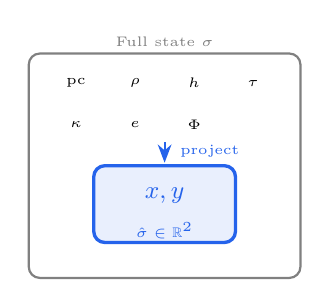
\begin{tikzpicture}[scale=0.75]
  % Full state
  \draw[thick, gray, rounded corners] (-0.3,-0.3) rectangle (4.3,3.5);
  \node[font=\tiny, gray] at (2,3.7) {Full state $\sigma$};
  
  \node[font=\tiny] at (0.5,3) {pc};
  \node[font=\tiny] at (1.5,3) {$\rho$};
  \node[font=\tiny] at (2.5,3) {$h$};
  \node[font=\tiny] at (3.5,3) {$\tau$};
  \node[font=\tiny] at (0.5,2.3) {$\kappa$};
  \node[font=\tiny] at (1.5,2.3) {$e$};
  \node[font=\tiny] at (2.5,2.3) {$\Phi$};
  
  % Projected
  \draw[very thick, accent, rounded corners, fill=accent!10] (0.8,0.3) rectangle (3.2,1.6);
  \node[font=\small\bfseries, accent] at (2,1.1) {$x, y$};
  \node[font=\tiny, accent] at (2,0.5) {$\hat\sigma \in \mathbb{R}^2$};
  
  % Arrow
  \draw[-{Stealth}, thick, accent] (2,2.0) -- (2,1.65);
  \node[font=\tiny, accent, right] at (2.1,1.85) {project};
\end{tikzpicture}
\end{center}
\vspace{0.3em}
\footnotesize
The ``heap model'' collapses to a flat $\mathbb{R}^2$: no pointers, no objects, no aliasing.
Constants $c, s$ are folded; loop index $i$ is universally quantified.
\end{column}
\end{columns}
\end{frame}


\begin{frame}{Stage 3b: Why Linear Abstractions Fail}
\begin{columns}[T]
\begin{column}{0.48\textwidth}
\begin{block}{The initial region}
\[
  S_0 = \{(x,y): x^2 + y^2 \ge 1\}
\]
This is the \emph{exterior of the unit disk}---it wraps
around the origin in every direction.
\end{block}

\vspace{0.3em}
\textbf{No halfplane} $ax + by \ge c > 0$ can contain~$S_0$
while excluding the origin.

\vspace{0.3em}
\textit{Proof:} For any $(a,b)$ with $a^2{+}b^2 > 0$,
the point $(-a/r, -b/r)$ with $r = \sqrt{a^2{+}b^2}$
lies on the unit circle (so $\in S_0$) but
$ax + by = -r < 0 < c$. \qed
\end{column}
\begin{column}{0.48\textwidth}
\begin{center}
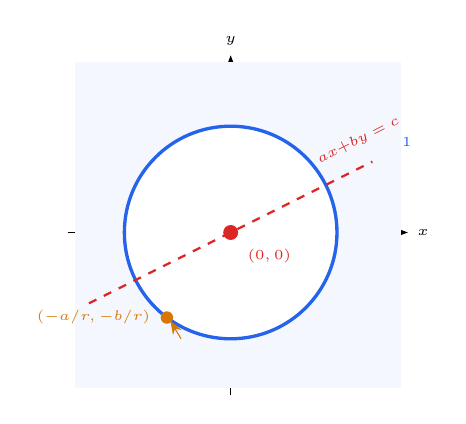
\begin{tikzpicture}[scale=0.9]
  % Axes
  \draw[-{Stealth}] (-2.3,0) -- (2.5,0) node[right,font=\tiny]{$x$};
  \draw[-{Stealth}] (0,-2.3) -- (0,2.5) node[above,font=\tiny]{$y$};

  % Unit circle (Init boundary)
  \draw[very thick, accent] (0,0) circle (1.5);
  \node[font=\tiny, accent] at (1.9,1.3) {$x^2{+}y^2=1$};

  % Exterior shading
  \fill[accent!5] (-2.2,-2.2) rectangle (2.4,2.4);
  \fill[white] (0,0) circle (1.5);
  
  % Redraw circle on top
  \draw[very thick, accent] (0,0) circle (1.5);
  
  % Origin (unsafe)
  \fill[unsafe] (0,0) circle (3pt);
  \node[font=\tiny, unsafe, below right] at (0.1,-0.1) {$(0,0)$};

  % Failed halfplane
  \draw[thick, unsafe, dashed] (-2,-1) -- (2,1);
  \node[font=\tiny, unsafe, rotate=27] at (1.8,1.3) {$ax{+}by=c$};

  % Arrow to counterexample on circle
  \fill[warn] (-0.9,-1.2) circle (2.5pt);
  \node[font=\tiny, warn, left] at (-1,-1.2) {$(-a/r,-b/r)$};
  \draw[-{Stealth}, thin, warn] (-0.7,-1.5) -- (-0.85,-1.25);
\end{tikzpicture}
\end{center}
\footnotesize
\begin{center}
Intervals, octagons, template polyhedra,\\
and CEGAR with linear predicates all\\
\textcolor{unsafe}{\textbf{provably fail}} on this program.
\end{center}
\end{column}
\end{columns}
\end{frame}


% ═══════════════════════════════════════════════════════════════════════════
%  PART IV — INFERRED BARRIER
% ═══════════════════════════════════════════════════════════════════════════

\begin{frame}{Stage 4: Inferred Barrier Certificate}
\begin{block}{Barrier template (degree 2)}
\vspace{-0.3em}
\[
  B(x, y) \;=\; c_0 + c_1\,x + c_2\,y + c_3\,x^2 + c_4\,xy + c_5\,y^2
\]
\end{block}

\vspace{0.3em}
\textbf{Three obligations} (Prajna--Jadbabaie 2004):
\begin{align}
  \text{(Init)}\quad & \forall (x,y) \in S_0:\; B(x,y) \ge \epsilon \label{eq:init}\\[4pt]
  \text{(Consecution)}\quad & \forall (x,y):\;
    B(x,y) \ge 0 \;\wedge\; T(x,y,x',y')
    \;\Rightarrow\; B(x',y') \ge 0 \label{eq:consec}\\[4pt]
  \text{(Separation)}\quad & \forall (x,y) \in U:\; B(x,y) \le -\epsilon \label{eq:sep}
\end{align}

\vspace{0.5em}
\begin{block}{Synthesized certificate (from Z3 template solving)}
\vspace{-0.3em}
\[
  \boxed{B(x, y) \;=\; x^2 + y^2 - 1}
  \qquad (c_3 = c_5 = 1,\; c_0 = -1,\; c_1 = c_2 = c_4 = 0)
\]
\end{block}
\end{frame}


\begin{frame}{Stage 4b: The Barrier Surface}
\begin{center}
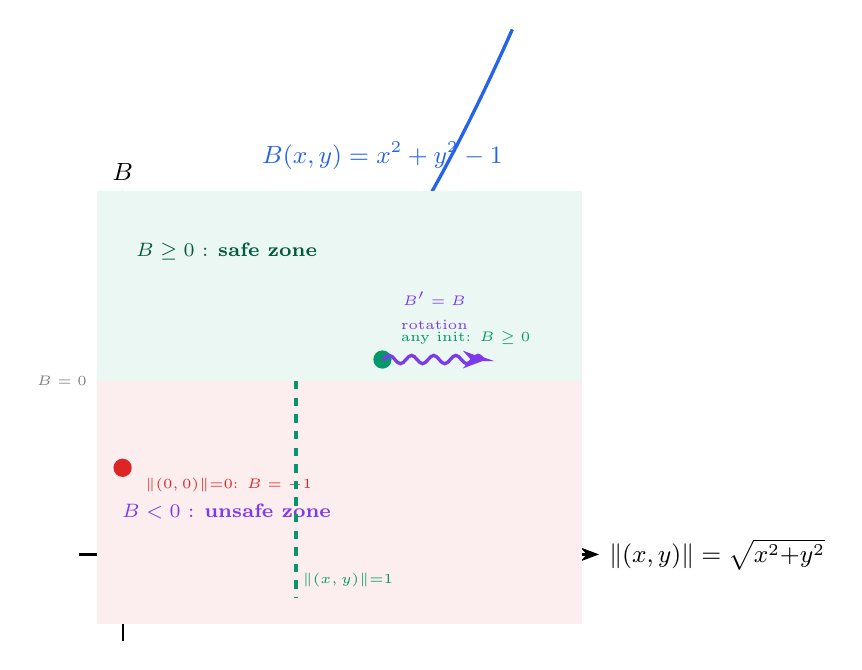
\begin{tikzpicture}[scale=1.1]
  \node[font=\small\bfseries, accent] at (3,4.6) {%
    $B(x,y) = x^2 + y^2 - 1$};

  % Axes
  \draw[-{Stealth}, thick] (-0.5,0) -- (5.5,0)
    node[right, font=\small]{$\|{(x,y)}\| = \sqrt{x^2{+}y^2}$};
  \draw[-{Stealth}, thick] (0,-1) -- (0,4.2) node[above, font=\small]{$B$};

  % Zero line
  \draw[gray, dashed] (-0.3,2) -- (5.3,2);
  \node[font=\tiny, gray, left] at (-0.3,2) {$B=0$};

  % B curve: B = r^2 - 1, plot in (r, B+2) for visibility
  % At r=0: B=-1, at r=1: B=0, at r=2: B=3
  \draw[very thick, accent, domain=0:4.5, samples=80]
    plot (\x, {2 + (\x/2)*(\x/2) - 1});

  % Regions
  \fill[safe!8] (-0.3,2) rectangle (5.3,4.2);
  \fill[unsafe!8] (-0.3,-0.8) rectangle (5.3,2);

  % Safe label
  \node[font=\scriptsize, safe!60!black] at (1.2,3.5)
    {$B \ge 0$ : \textbf{safe zone}};
  \node[font=\scriptsize, fence] at (1.2,0.5)
    {$B < 0$ : \textbf{unsafe zone}};

  % Unsafe point (origin)
  \fill[unsafe] (0,1) circle (3pt);
  \node[font=\tiny, unsafe, right] at (0.15,0.8)
    {$\|(0,0)\|{=}0$: $B=-1$};

  % Init region boundary
  \draw[very thick, safe, dashed] (2,2) -- (2,-0.5);
  \node[font=\tiny, safe] at (2.6,-0.3) {$\|{(x,y)}\|{=}1$};

  % Safe point
  \fill[safe] (3,2.25) circle (3pt);
  \node[font=\tiny, safe, right] at (3.1,2.5)
    {any init: $B \ge 0$};

  % Arrow showing rotation preserves
  \draw[-{Stealth}, very thick, hilbert, decorate,
    decoration={snake, amplitude=1.5pt, segment length=8pt}]
    (3,2.25) -- (4.2,2.25);
  \node[font=\tiny, hilbert] at (3.6,2.65) {rotation};
  \node[font=\tiny, hilbert] at (3.6,2.95) {$B' = B$};
\end{tikzpicture}
\end{center}

\vspace{0.3em}
\footnotesize
The barrier is \textbf{exactly invariant} under the rotation ($B' = B$),
so any state starting with $B \ge 0$ can never reach $B < 0$.
\end{frame}


\begin{frame}{Stage 4c: Why $B$ Is Exactly Preserved}
\begin{block}{Algebraic proof (confirmed by Z3)}
Let $x' = cx - sy$, $y' = sx + cy$ with $c = 3/5$, $s = 4/5$.\\[6pt]
Then:
\begin{align*}
  x'^2 + y'^2 &= (cx - sy)^2 + (sx + cy)^2 \\[4pt]
  &= c^2 x^2 - 2csxy + s^2 y^2 + s^2 x^2 + 2csxy + c^2 y^2 \\[4pt]
  &= \underbrace{(c^2 + s^2)}_{=\,1}\,x^2 + \underbrace{(s^2 + c^2)}_{=\,1}\,y^2 \\[4pt]
  &= x^2 + y^2
\end{align*}
\end{block}

Therefore:
\[
  B(x', y') = x'^2 + y'^2 - 1 = x^2 + y^2 - 1 = B(x, y)
\]

\vspace{0.3em}
\begin{center}
\fbox{\parbox{0.7\textwidth}{\centering\small
  The cross-terms $-2csxy$ and $+2csxy$ cancel exactly.\\
  This is why \textbf{nonlinear arithmetic} is essential:\\
  a linear solver cannot discover this cancellation.
}}
\end{center}
\end{frame}


% ═══════════════════════════════════════════════════════════════════════════
%  PART V — SMT OBLIGATIONS
% ═══════════════════════════════════════════════════════════════════════════

\begin{frame}[fragile]{Stage 5: SMT Obligations (Z3 Discharge)}
\begin{block}{What A3 sends to Z3: three negated queries (should all be UNSAT)}
\end{block}

\vspace{0.3em}
\footnotesize
\textbf{Obligation 1 --- Init} (should be UNSAT):
\begin{align*}
  \exists\, x, y \in \mathbb{R}:\quad
  & x^2 + y^2 \ge 1 \;\wedge\; (x^2 + y^2 - 1) < 0
\end{align*}
\begin{center}
\texttt{Z3 result: \textcolor{safe}{\textbf{unsat}}} \quad $\Rightarrow$ \textcolor{safe}{\faCheck\; PASS}
\end{center}

\vspace{0.3em}
\textbf{Obligation 2 --- Consecution} (should be UNSAT):
\begin{align*}
  \exists\, x, y:\quad
  & x^2 + y^2 - 1 \ge 0 \;\wedge\;
    \bigl(\tfrac{3}{5}x - \tfrac{4}{5}y\bigr)^2 + \bigl(\tfrac{4}{5}x + \tfrac{3}{5}y\bigr)^2 - 1 < 0
\end{align*}
\begin{center}
\texttt{Z3 result: \textcolor{safe}{\textbf{unsat}}} \quad $\Rightarrow$ \textcolor{safe}{\faCheck\; PASS}
\end{center}

\vspace{0.3em}
\textbf{Obligation 3 --- Separation} (should be UNSAT):
\begin{align*}
  \exists\, x, y:\quad
  & x = 0 \;\wedge\; y = 0 \;\wedge\; (x^2 + y^2 - 1) \ge 0
\end{align*}
\begin{center}
\texttt{Z3 result: \textcolor{safe}{\textbf{unsat}}} \quad $\Rightarrow$ \textcolor{safe}{\faCheck\; PASS}
\end{center}
\end{frame}


\begin{frame}{Stage 5b: Additional Z3 Confirmations}
\begin{block}{Algebraic side-obligations (also discharged by Z3)}
\end{block}

\vspace{0.3em}
\renewcommand{\arraystretch}{1.6}
\begin{tabular}{@{}lp{7cm}c@{}}
\toprule
\textbf{Check} & \textbf{Z3 Query} & \textbf{Result} \\
\midrule
$c^2 + s^2 = 1$ &
  $\exists\, c{=}\tfrac{3}{5}, s{=}\tfrac{4}{5}:\; c^2{+}s^2 \ne 1$
  & \textcolor{safe}{\texttt{unsat} \faCheck} \\
$B' = B$ exactly &
  $\exists\, x,y:\; B(x',y') - B(x,y) \ne 0$
  & \textcolor{safe}{\texttt{unsat} \faCheck} \\
$B(0,0) = -1$ &
  Evaluate: $0^2 + 0^2 - 1 = -1 < 0$
  & \textcolor{safe}{\faCheck} \\
\bottomrule
\end{tabular}

\vspace{0.5em}
\begin{center}
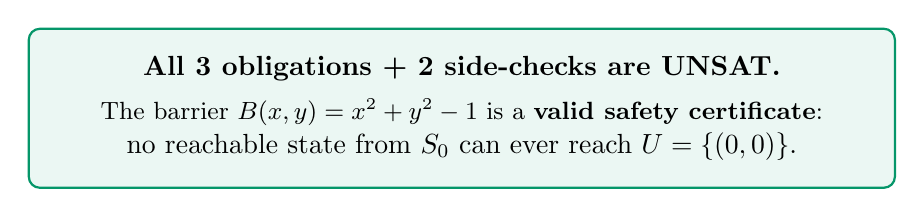
\begin{tikzpicture}
  \node[draw, rounded corners, fill=safe!8, thick, draw=safe,
        minimum width=11cm, align=center, inner sep=10pt] {
    \textbf{All 3 obligations + 2 side-checks are UNSAT.}\\[4pt]
    \small
    The barrier $B(x,y) = x^2 + y^2 - 1$ is a \textbf{valid safety certificate}:\\
    no reachable state from $S_0$ can ever reach $U = \{(0,0)\}$.
  };
\end{tikzpicture}
\end{center}
\end{frame}


\begin{frame}{Stage 5c: SOS / Positivstellensatz View}
\begin{block}{Putinar's Positivstellensatz (the engine under the hood)}
If $B(\mathbf{x}) \ge 0$ on $\{g_1 \ge 0, \ldots, g_m \ge 0\}$, then:
\[
  B = s_0 + s_1 g_1 + \cdots + s_m g_m
  \quad\text{where each $s_i$ is \textbf{sum-of-squares}}
\]
\end{block}

\vspace{0.3em}
For our rotation barrier:

\begin{align}
  \text{(Init):}\quad & B\big|_{S_0} \;=\; \underbrace{0}_{\text{SOS}} +
    \underbrace{1}_{= 1^2\text{, SOS}} \cdot \underbrace{(x^2{+}y^2 - 1)}_{g_{\mathrm{init}}} \\[6pt]
  \text{(Sep):}\quad & -B\big|_{U} \;=\; -(0 + 0 - 1) \;=\; 1 \;=\; \underbrace{1^2}_{\text{SOS}} \\[6pt]
  \text{(Consec):}\quad & B(x',y') - B(x,y) \;=\; 0 \;=\; \underbrace{0}_{\text{SOS}}
\end{align}

\vspace{0.3em}
\footnotesize
Every multiplier is trivially SOS.
This is a particularly clean example: the barrier is an \textbf{exact invariant} ($B' = B$),
so consecution reduces to $0 = 0$.
\end{frame}


% ═══════════════════════════════════════════════════════════════════════════
%  PART VI — BUG REPORT
% ═══════════════════════════════════════════════════════════════════════════

\begin{frame}{Stage 6: Bug Report (With Precondition)}
\begin{center}
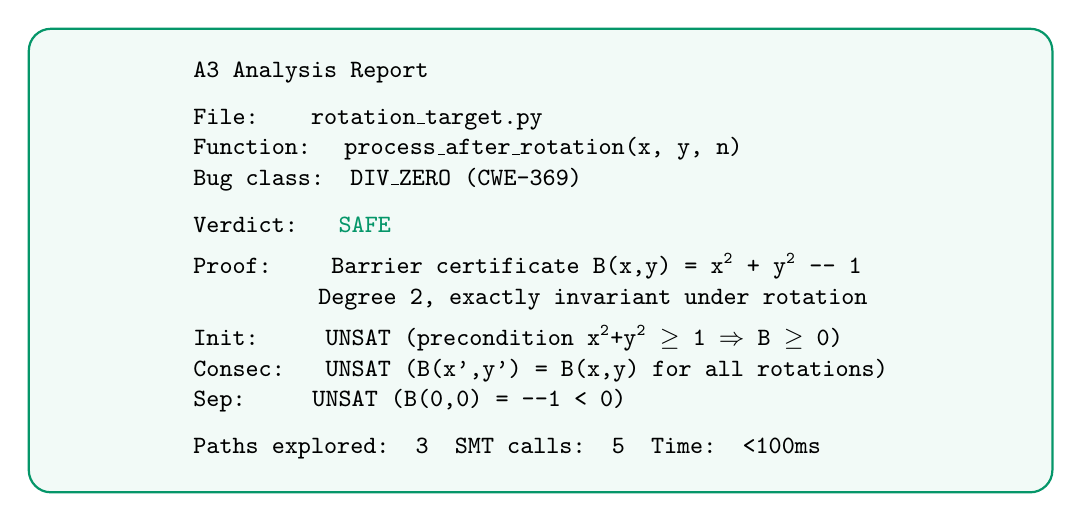
\begin{tikzpicture}
  \node[draw, thick, rounded corners=8pt, fill=safe!5, draw=safe,
        minimum width=13cm, minimum height=4cm, align=left, inner sep=12pt,
        font=\small] {
    \texttt{\textbf{A3 Analysis Report}}\\[6pt]
    \texttt{File:\quad\quad rotation\_target.py}\\
    \texttt{Function:\; process\_after\_rotation(x, y, n)}\\
    \texttt{Bug class: DIV\_ZERO (CWE-369)}\\[6pt]
    \texttt{Verdict:\;\; \textcolor{safe}{\textbf{SAFE}}}\\[4pt]
    \texttt{Proof:\quad\; Barrier certificate B(x,y) = x\textsuperscript{2} + y\textsuperscript{2} -- 1}\\
    \texttt{\phantom{Proof:\quad\;} Degree 2, exactly invariant under rotation}\\[4pt]
    \texttt{Init:\quad\;\; UNSAT (precondition x\textsuperscript{2}+y\textsuperscript{2} $\ge$ 1 $\Rightarrow$ B $\ge$ 0)}\\
    \texttt{Consec:\;\; UNSAT (B(x',y') = B(x,y) for all rotations)}\\
    \texttt{Sep:\quad\;\; UNSAT (B(0,0) = --1 < 0)}\\[6pt]
    \texttt{Paths explored: 3\quad SMT calls: 5\quad Time: <100ms}
  };
\end{tikzpicture}
\end{center}
\end{frame}


\begin{frame}{Stage 6b: What If the Precondition Is Removed?}
\begin{columns}[T]
\begin{column}{0.52\textwidth}
\begin{block}{Without $x^2 + y^2 \ge 1$}
If we allow \emph{any} $(x,y)$ as input, then $(0,0)$ is a valid initial state.

\vspace{0.3em}
After any number of rotations:
\[
  x' = 0,\quad y' = 0 \quad\Rightarrow\quad x'^2 + y'^2 = 0
\]
\[
  \texttt{1.0 / 0} \;\to\; \textcolor{unsafe}{\textbf{ZeroDivisionError}}
\]
\end{block}

\vspace{0.3em}
The barrier Init obligation \textbf{fails}:
\[
  B(0,0) = -1 < 0 \quad\text{but $(0,0) \in S_0$}
\]
\end{column}
\begin{column}{0.44\textwidth}
\begin{center}
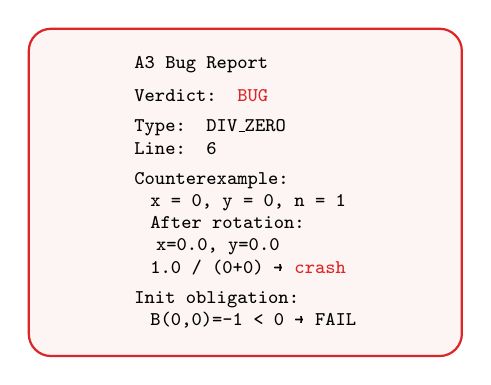
\begin{tikzpicture}
  \node[draw, thick, rounded corners=8pt, fill=unsafe!5, draw=unsafe,
        minimum width=5.5cm, minimum height=3.5cm, align=left, inner sep=10pt,
        font=\scriptsize] {
    \texttt{\textbf{A3 Bug Report}}\\[4pt]
    \texttt{Verdict: \textcolor{unsafe}{\textbf{BUG}}}\\[3pt]
    \texttt{Type: DIV\_ZERO}\\
    \texttt{Line: 6}\\[3pt]
    \texttt{Counterexample:}\\
    \texttt{\; x = 0, y = 0, n = 1}\\
    \texttt{\; After rotation:}\\
    \texttt{\;\; x=0.0, y=0.0}\\
    \texttt{\; 1.0 / (0+0) → \textcolor{unsafe}{crash}}\\[3pt]
    \texttt{Init obligation:}\\
    \texttt{\; B(0,0)=-1 < 0 → FAIL}
  };
\end{tikzpicture}
\end{center}
\end{column}
\end{columns}
\end{frame}


% ═══════════════════════════════════════════════════════════════════════════
%  COMPARISON: WHY BARRIERS
% ═══════════════════════════════════════════════════════════════════════════

\begin{frame}{Why a Barrier? Comparison of Approaches}
\begin{center}
\begin{tikzpicture}[
  approach/.style={draw, rounded corners=6pt, thick, minimum width=3.6cm,
                   minimum height=3.2cm, align=center, font=\small, inner sep=8pt},
]
  \node[approach, fill=unsafe!5, draw=unsafe] (lin) at (0,0) {
    \textbf{Linear Abstractions}\\
    \textbf{(Intervals / Polyhedra)}\\[6pt]
    \scriptsize
    Invariant: $ax + by \ge c$\\[3pt]
    \textcolor{unsafe}{\faTimes\; Cannot enclose $x^2{+}y^2 \ge 1$}\\
    \textcolor{unsafe}{\faTimes\; All halfplanes miss part}\\
    \textcolor{unsafe}{\faTimes\; of the unit circle}\\
    \textcolor{safe}{\faCheck\; Fast}
  };

  \node[approach, fill=warn!5, draw=warn] (mc) at (5,0) {
    \textbf{Explicit-State}\\
    \textbf{Model Checking}\\[6pt]
    \scriptsize
    Enumerate reachable states\\[3pt]
    \textcolor{unsafe}{\faTimes\; $x,y \in \mathbb{R}$ = infinite}\\
    \textcolor{unsafe}{\faTimes\; Cannot enumerate $\mathbb{R}^2$}\\
    \textcolor{unsafe}{\faTimes\; No compact proof}\\
    \textcolor{safe}{\faCheck\; Sound if finite}
  };

  \node[approach, fill=hilbert!5, draw=hilbert] (bar) at (10,0) {
    \textbf{Quadratic Barrier}\\
    \textbf{(A3 approach)}\\[6pt]
    \scriptsize
    $B = x^2 + y^2 - 1$\\[3pt]
    \textcolor{safe}{\faCheck\; Handles curved init set}\\
    \textcolor{safe}{\faCheck\; SOS/SMT verified}\\
    \textcolor{safe}{\faCheck\; Works for all $n$}\\
    \textcolor{safe}{\faCheck\; Compact certificate}
  };

  \draw[very thick, hilbert, rounded corners=8pt]
    (bar.south west) +(-0.15,-0.15)
    rectangle ([shift={(0.15,0.15)}]bar.north east);
\end{tikzpicture}
\end{center}
\end{frame}


% ═══════════════════════════════════════════════════════════════════════════
%  SUMMARY PIPELINE
% ═══════════════════════════════════════════════════════════════════════════

\begin{frame}{Summary: The Complete Pipeline}
\begin{center}
\begin{tikzpicture}[
  step/.style={draw, rounded corners, thick, fill=#1!10, draw=#1,
               minimum width=13cm, minimum height=0.85cm, align=left,
               font=\small, inner xsep=8pt},
  arr/.style={-{Stealth[length=4pt]}, thick, gray}
]
  \node[step=gray] (s1) at (0,5) {
    \textbf{1.} Source: \texttt{process\_after\_rotation(x, y, n)} $\to$ 6 locals, 23 bytecodes
  };
  \node[step=accent] (s2) at (0,4) {
    \textbf{2.} Transition system: $\hat\sigma = (x,y)$, \;Trans: $(x,y) \mapsto (cx{-}sy,\; sx{+}cy)$
  };
  \node[step=hilbert] (s3) at (0,3) {
    \textbf{3.} Heap model: no heap ($h = \emptyset$), project to $\mathbb{R}^2$
  };
  \node[step=fence] (s4) at (0,2) {
    \textbf{4.} Barrier: $B(x,y) = x^2 + y^2 - 1$ \;\;(degree 2, exactly invariant)
  };
  \node[step=verify] (s5) at (0,1) {
    \textbf{5.} SMT: Init \textcolor{safe}{\faCheck}\; Consecution \textcolor{safe}{\faCheck}\; Separation \textcolor{safe}{\faCheck}\; $c^2{+}s^2{=}1$ \textcolor{safe}{\faCheck}\; $B'{=}B$ \textcolor{safe}{\faCheck}
  };
  \node[step=safe] (s6) at (0,0) {
    \textbf{6.} Verdict: \textcolor{safe}{\textbf{SAFE}} --- division by zero unreachable under precondition
  };

  \foreach \i/\j in {s1/s2, s2/s3, s3/s4, s4/s5, s5/s6} {
    \draw[arr] (\i.south) -- (\j.north);
  }
\end{tikzpicture}
\end{center}
\end{frame}


\begin{frame}{Key Takeaway}
\begin{center}
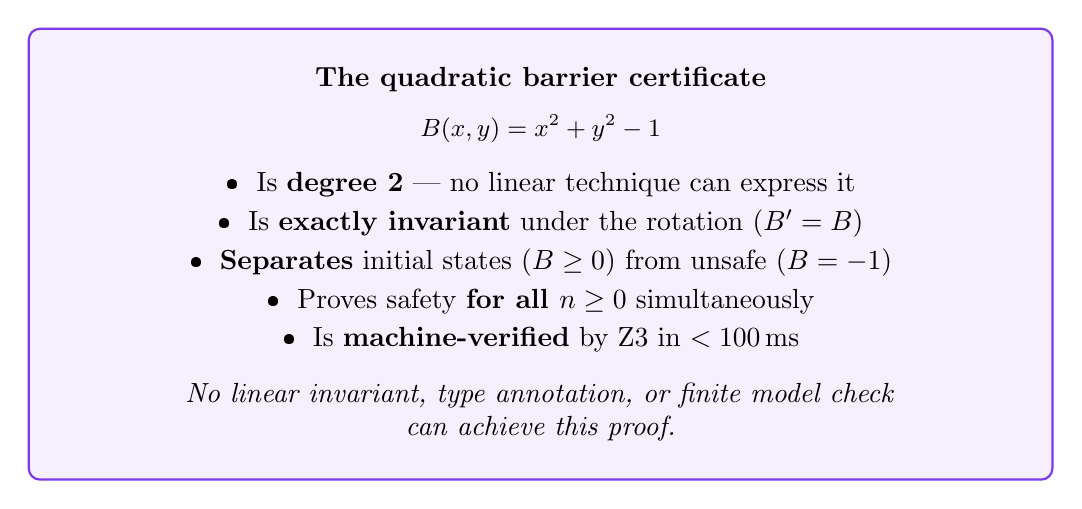
\begin{tikzpicture}
  \node[draw, rounded corners, fill=hilbert!8, thick, draw=hilbert,
        minimum width=13cm, align=center, inner sep=14pt] {
    \textbf{The quadratic barrier certificate}\\[6pt]
    \small
    $B(x,y) = x^2 + y^2 - 1$\\[8pt]
    \textbullet\; Is \textbf{degree 2} --- no linear technique can express it\\[2pt]
    \textbullet\; Is \textbf{exactly invariant} under the rotation ($B' = B$)\\[2pt]
    \textbullet\; \textbf{Separates} initial states ($B \ge 0$) from unsafe ($B = -1$)\\[2pt]
    \textbullet\; Proves safety \textbf{for all $n \ge 0$} simultaneously\\[2pt]
    \textbullet\; Is \textbf{machine-verified} by Z3 in $< 100$\,ms\\[8pt]
    \normalsize
    \textit{No linear invariant, type annotation, or finite model check}\\
    \textit{can achieve this proof.}
  };
\end{tikzpicture}
\end{center}
\end{frame}


\begin{frame}[plain]
\begin{center}
\vspace{2cm}
{\Huge\textcolor{accent}{\textbf{fin}}}

\vspace{1cm}
{\large Source $\to$ Transition System $\to$ Heap Model $\to$ Barrier $\to$ SMT $\to$ Proof}

\vspace{0.5cm}
{\small Built on: Prajna--Jadbabaie 2004 (barriers),\;
Putinar (Positivstellensatz),\; Z3 (SMT)}

\vspace{0.3cm}
{\footnotesize All Z3 queries executed by
\texttt{scripts/rotation\_pipeline\_instrument.py}}
\end{center}
\end{frame}

\end{document}
